\chapter{Ácidos e bases: Ka e pKa}\label{ch:g12:ka-and-pka}

Muitas formigas se defendem com ácido metanoico, e na pele ele queima. O
ácido metanoico é um \omterm{def:g11:functional-groups:carboxylic-acid}{ácido carboxílico} pequeno. O ácido clorídrico na
mesma concentração queimaria muito mais. Os dois são ácidos; os dois dão
uma solução de \omterm{def:g9:acids-bases-ph:ph}{pH} abaixo de 7; no entanto, eles não são ácidos da mesma
maneira. Para descrever completamente um ácido, são necessários dois
números: quanto há dele, a sua concentração, e com que facilidade ele
cede o seu \omterm{def:g9:ions:ion}{íon} hidrogênio, a sua \omterm{def:g12:ka-and-pka:ka}{constante de acidez}.

\begin{recall}
As \omterm{def:g9:acids-bases-ph:acidic}{soluções ácidas}, básicas e neutras; a escala de \omterm{def:g9:acids-bases-ph:ph}{pH}, de 0 a 14, mais
baixa quando há mais \omterm{def:g9:ions:ion}{íons} hidrogênio (\cref{ch:g9:acids-bases-ph}). O
\omterm{def:g12:equilibrium:quotient}{quociente de reação} $Q$ e a \omterm{def:g12:equilibrium:constant}{constante de equilíbrio} $K$
(\cref{ch:g12:equilibrium}). Uma \omterm{def:g12:curly-arrows:curly-arrow}{seta curva} mostra um par de \omterm{def:g9:inside-the-atom:nucleus}{elétrons} se
deslocando (\cref{ch:g12:curly-arrows}).
\end{recall}

\begin{omfigure}
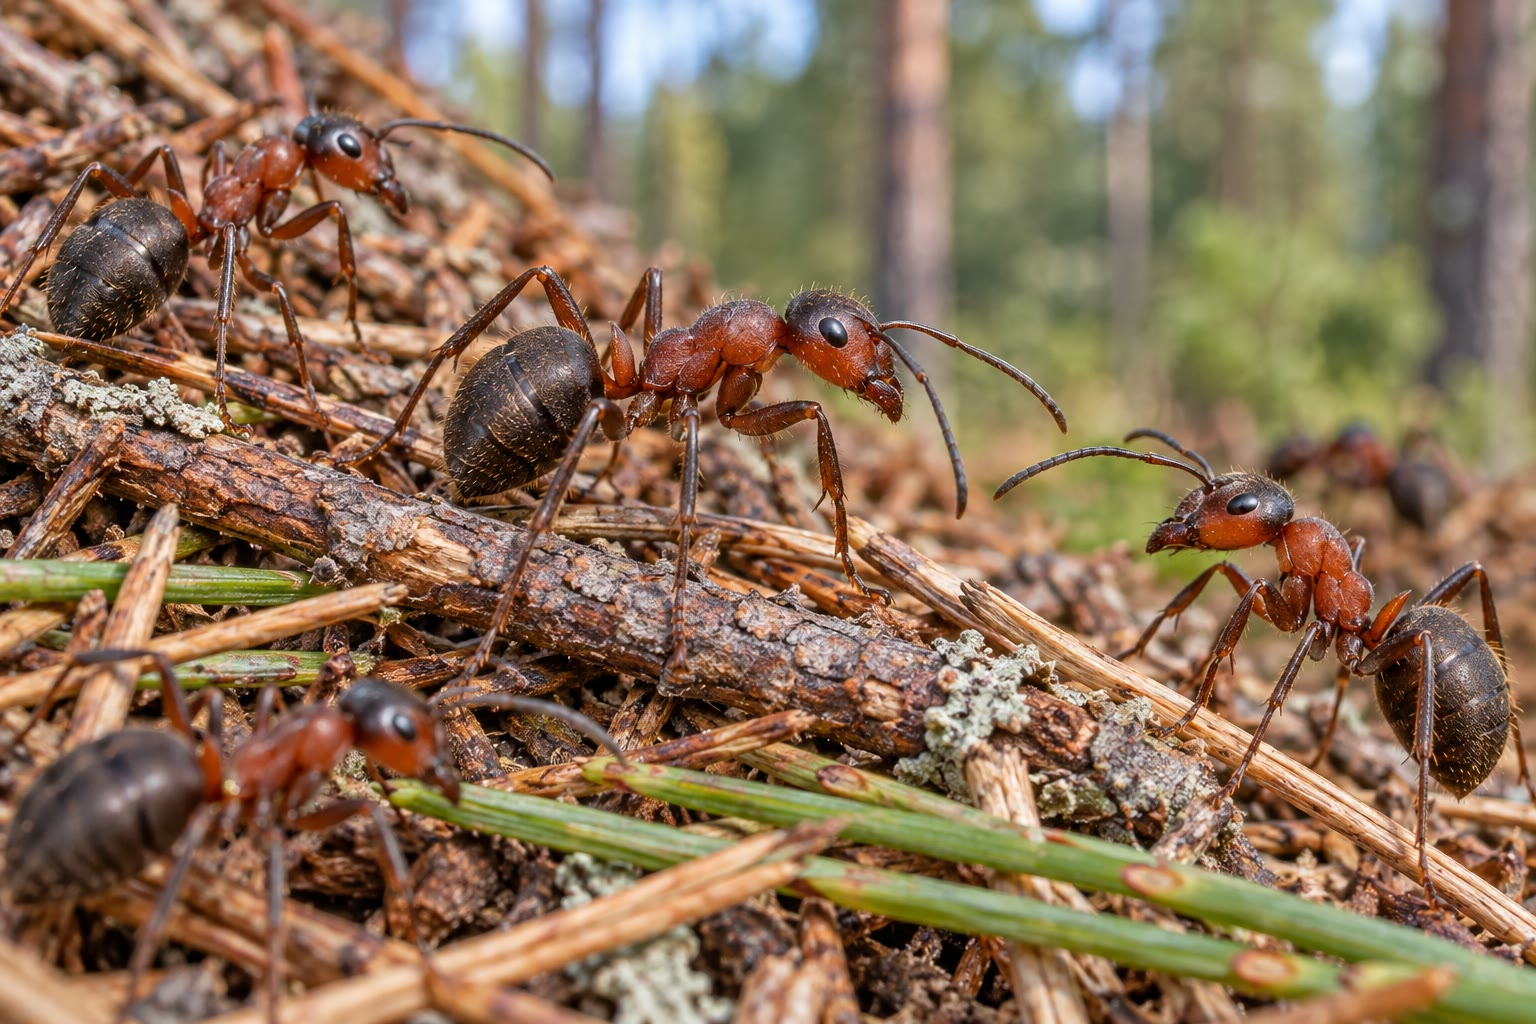
\includegraphics[width=0.45\linewidth]{images/book1/ai/g12-red-ants.jpg}

{\small Formigas-ruivas: como muitas formigas, elas se defendem com ácido metanoico.}
\end{omfigure}

\section{Os ácidos e as bases de Brønsted}

\begin{definition}[Ácido e base de Brønsted, par ácido--base]\label{def:g12:ka-and-pka:bronsted}
Um \emph{ácido de Brønsted}\index{acido de Brnsted@ácido de Brønsted} é uma espécie capaz
de ceder um \omterm{def:g9:ions:ion}{íon} hidrogênio \ce{H+}; uma \emph{base de
Brønsted}\index{base de Brnsted@base de Brønsted} é uma espécie capaz de captar um. Um
ácido HA e a base \ce{A-} em que ele se transforma ao perder \ce{H+}
formam um \emph{par ácido--base}\index{par acido--base@par ácido--base}, escrito
\ce{HA}/\ce{A-}: $\ce{HA} \rightleftharpoons \ce{A-} + \ce{H+}$.
\end{definition}

\begin{definition}[Íon oxônio, espécie anfótera]\label{def:g12:ka-and-pka:oxonium}
Na água, um \omterm{def:g9:ions:ion}{íon} hidrogênio nunca fica sozinho: ele é captado por uma
\omterm{def:g7:atoms-and-molecules:molecule}{molécula} de água, o que dá o \emph{íon oxônio}\index{ion oxonio@íon oxônio}
\ce{H3O+}. Uma espécie que é o ácido de um par e a base de outro é uma
\emph{espécie anfótera}\index{especie anfotera@espécie anfótera}; a água é uma delas,
ácido do par \ce{H2O}/\ce{OH-} e base do par \ce{H3O+}/\ce{H2O}.
\end{definition}

\begin{example}[Um ácido na água]\label{ex:g12:ka-and-pka:acid-water}
Quando o ácido etanoico \omterm{def:g2:mixing-and-dissolving:dissolve}{se dissolve}, um \omterm{def:g10:lewis-and-shape:lone-pair}{par não ligante} de uma \omterm{def:g7:atoms-and-molecules:molecule}{molécula}
de água capta o hidrogênio do seu \ce{O-H}, e o par \ce{O-H} fica no
oxigênio do ácido:
\[
  \ce{CH3COOH + H2O <=> CH3COO- + H3O+} .
\]
Dois pares trocam um \omterm{def:g9:ions:ion}{íon} hidrogênio: \ce{CH3COOH}/\ce{CH3COO-} o cede,
\ce{H3O+}/\ce{H2O} o capta. De agora em diante, os \omterm{def:g9:ions:ion}{íons} hidrogênio dos
capítulos anteriores são escritos \ce{H3O+} sempre que a água é o
\omterm{def:g6:solutions-and-solubility:solute}{solvente}.
\end{example}

\begin{omfigure}
\setchemfig{atom sep=2em}
\chemfig{H_3C-C(=[2]O)-O-[@{oh}]@{h}H}\qquad
\chemfig{@{ow}\charge{90=\:,270=\:}{O}(-[:150]H)-[:210]H}
\qquad$\longrightarrow$\qquad
\chemfig{H_3C-C(=[2]O)-\charge{90=\:,0=\:,270=\:}{O}^{-}}\quad$+$\quad\ce{H3O+}
\chemmove{
  \draw[->, thick, omProp, shorten <=4pt, shorten >=3pt]
    ($(ow)+(0,0.25)$) .. controls +(110:9mm) and +(60:9mm) .. (h);
  \draw[->, thick, omDef, shorten <=2pt, shorten >=4pt]
    (oh) .. controls +(-90:7mm) and +(-60:6mm) .. ($(oh)+(-0.3,-0.2)$);}

{\small Um \omterm{def:g9:ions:ion}{íon} hidrogênio passa do ácido para a água: um \omterm{def:g10:lewis-and-shape:lone-pair}{par não ligante}
da água forma a nova ligação \ce{O-H} (em laranja), e o antigo par
\ce{O-H} fica no oxigênio do \omterm{def:g9:ions:ion}{íon} etanoato (em azul).}
\end{omfigure}

\begin{history}[De Arrhenius a Brønsted, 1887--1923]
Em 1887, Svante Arrhenius propôs que os ácidos dão \omterm{def:g9:ions:ion}{íons} hidrogênio na
água e as bases, \omterm{def:g9:ions:ion}{íons} hidróxido. Em 1923, Johannes Brønsted e,
independentemente, Thomas Lowry ampliaram a ideia: um ácido é qualquer
espécie que cede um \omterm{def:g9:ions:ion}{íon} hidrogênio, uma base qualquer espécie que capta
um, na água ou não. A \omterm{def:g7:atoms-and-molecules:molecule}{molécula} de amônia, que não contém hidróxido,
virou uma base como qualquer outra.
\end{history}

\begin{omfigure}
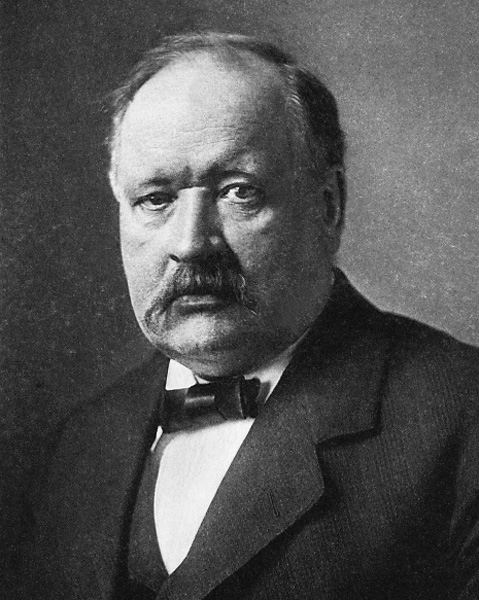
\includegraphics[width=0.22\linewidth]{images/book1/arrhenius.jpg}

{\small Svante Arrhenius (1859--1927).}
\end{omfigure}

\section{O pH, quantitativamente}

\begin{definition}[O pH, com precisão]\label{def:g12:ka-and-pka:ph-log}
Numa \omterm{def:g6:solutions-and-solubility:solute}{solução aquosa} diluída, o \omterm{def:g9:acids-bases-ph:ph}{pH} é definido por
\[
  \mathrm{pH} = -\log\frac{[\ce{H3O+}]}{c^\circ},
  \qquad\text{isto é}\qquad
  [\ce{H3O+}] = c^\circ \times 10^{-\mathrm{pH}} ,
\]
em que $\log$ é o logaritmo decimal.
\end{definition}

\begin{proposition}[Diluição por dez, uma unidade]\label{prop:g12:ka-and-pka:dilution}
Se $[\ce{H3O+}]$ é dividida por 10, o \omterm{def:g9:acids-bases-ph:ph}{pH} aumenta 1; se ela é
multiplicada por 10, o \omterm{def:g9:acids-bases-ph:ph}{pH} diminui 1.
\end{proposition}

\begin{proof}
$-\log\big([\ce{H3O+}]/10c^\circ\big) = -\log\big([\ce{H3O+}]/c^\circ\big)
+ \log 10 = \mathrm{pH} + 1$.
\end{proof}

\begin{definition}[Ácidos e bases fortes e fracos]\label{def:g12:ka-and-pka:strong-acid}
Um \emph{ácido forte}\index{acido forte@ácido forte} reage totalmente com a água:
nada do ácido continua como tal na solução. Um \emph{ácido
fraco}\index{acido fraco@ácido fraco} reage parcialmente: a sua reação com a água
chega a um equilíbrio. Da mesma forma, uma \emph{base
forte}\index{base forte} reage totalmente com a água, uma \emph{base
fraca}\index{base fraca} parcialmente.
\end{definition}

\begin{proposition}[O pH de um ácido forte]\label{prop:g12:ka-and-pka:strong}
Uma solução de um \omterm{def:g12:ka-and-pka:strong-acid}{ácido forte} de concentração $c$ (não diluída demais)
tem $[\ce{H3O+}] = c$ e $\mathrm{pH} = -\log(c/c^\circ)$.
\end{proposition}

\begin{proof}
A reação \ce{HA + H2O -> A- + H3O+} é total: cada \omterm{def:g7:atoms-and-molecules:molecule}{molécula} de ácido dá
um \omterm{def:g12:ka-and-pka:oxonium}{íon oxônio}. Os \omterm{def:g9:ions:ion}{íons} que vêm da própria água são desprezíveis enquanto
$c$ for muito maior que \qty{e-7}{mol/L}.
\end{proof}

\begin{example}[O ácido clorídrico]\label{ex:g12:ka-and-pka:hcl}
Ácido clorídrico a \qty{0.010}{mol/L}: $[\ce{H3O+}] = \qty{0.010}{mol/L}$
e $\mathrm{pH} = -\log 0.010 = 2.0$. Diluído dez vezes, \omterm{def:g9:acids-bases-ph:ph}{pH} 3.0.
\end{example}

\section{A água e o produto iônico}


\begin{definition}[Produto iônico da água]\label{def:g12:ka-and-pka:ionic-product}
A água reage muito pouco consigo mesma, \ce{2H2O <=> H3O+ + OH-}. A
\omterm{def:g12:equilibrium:constant}{constante de equilíbrio} dessa reação é o \emph{produto iônico da
água}\index{produto ionico da agua@produto iônico da água}:
\[
  K_e = \frac{[\ce{H3O+}]\,[\ce{OH-}]}{(c^\circ)^2},
  \qquad pK_e = -\log K_e .
\]
\end{definition}

\begin{proposition}[A água neutra e as bases fortes]\label{prop:g12:ka-and-pka:ke}
% ledger: ke:25C
A \qty{25}{\celsius}, $K_e = \num{1.0e-14}$ e $pK_e = 14.0$. Na água
pura, $[\ce{H3O+}] = [\ce{OH-}] = \qty{1.0e-7}{mol/L}$: \omterm{def:g9:acids-bases-ph:ph}{pH} 7.0. Uma \omterm{def:g12:ka-and-pka:strong-acid}{base
forte} de concentração $c$ dá $[\ce{OH-}] = c$, logo
$[\ce{H3O+}] = K_e (c^\circ)^2 / c$ e $\mathrm{pH} = 14.0 + \log(c/c^\circ)$.
\end{proposition}

\begin{proof}
Na água pura, os dois \omterm{def:g9:ions:ion}{íons} vêm aos pares, logo são iguais, e o seu
produto é $\num{1.0e-14}$: cada um vale \qty{1.0e-7}{mol/L}. Para a base,
$K_e$ continua valendo na solução:
$-\log([\ce{H3O+}]/c^\circ) = -\log K_e + \log(c/c^\circ)$.
\end{proof}

\begin{example}[O hidróxido de sódio]\label{ex:g12:ka-and-pka:naoh}
Hidróxido de sódio a \qty{0.010}{mol/L}: $[\ce{OH-}] = 0.010$, logo
$[\ce{H3O+}] = \num{1.0e-14}/0.010 = \qty{1.0e-12}{mol/L}$ e \omterm{def:g9:acids-bases-ph:ph}{pH} 12.0.
\end{example}

\section{A constante de acidez}

\begin{definition}[Constante de acidez, $pK_a$]\label{def:g12:ka-and-pka:ka}
A \emph{constante de acidez}\index{constante de acidez} $K_a$ de um par
\ce{HA}/\ce{A-} é a \omterm{def:g12:equilibrium:constant}{constante de equilíbrio} da reação do ácido com a
água, \ce{HA + H2O <=> A- + H3O+}:
\[
  K_a = \frac{[\ce{A-}]\,[\ce{H3O+}]}{[\ce{HA}]\,c^\circ} .
\]
O \emph{pKa}\index{pKa} do par é
$pK_a = -\log K_a$.
\end{definition}

\begin{proposition}[Quanto menor o $pK_a$, mais forte o ácido]\label{prop:g12:ka-and-pka:compare}
De dois \omterm{def:g12:ka-and-pka:strong-acid}{ácidos fracos} na mesma concentração, aquele que tem o maior
$K_a$, isto é, o menor $pK_a$, reage mais com a água e dá o \omterm{def:g9:acids-bases-ph:ph}{pH} mais
baixo; a sua base conjugada é a mais fraca.
\end{proposition}

\begin{proof}
Um $K_a$ maior significa mais \ce{A-} e \ce{H3O+} no equilíbrio para o
mesmo \ce{HA}. A base \ce{A-} de um par que cede facilmente o seu \omterm{def:g9:ions:ion}{íon}
hidrogênio só o recupera com relutância.
\end{proof}

\begin{omfigure}
\begin{tikzpicture}[font=\small, y=0.55cm]
  % ledger: pka:methanoic, pka:ethanoic, pka:benzoic, pka:ascorbic1, ka:HF, ka:H2CO3, ka:HCO3, kb:NH3, ke:25C
  \draw[->, thick] (0,0) -- (0,14.8) node[above] {$pK_a$};
  \foreach \k in {0,2,4,6,8,10,12,14} \draw (-0.1,\k) -- (0.1,\k) node[right, font=\scriptsize] {\k};
  \node[font=\footnotesize\bfseries, anchor=south] at (-3.0,14.3) {ácido};
  \node[font=\footnotesize\bfseries, anchor=south] at (3.0,14.3) {base};
  \foreach \p/\yl/\acid/\base in {3.19/2.9/{\ce{HF}}/{\ce{F-}},
      3.74/3.6/{\ce{HCOOH}}/{\ce{HCOO-}}, 4.04/4.3/{ácido ascórbico}/{ascorbato},
      4.20/5.0/{\ce{C6H5COOH}}/{\ce{C6H5COO-}}, 4.76/5.7/{\ce{CH3COOH}}/{\ce{CH3COO-}},
      6.37/6.9/{\ce{CO2,H2O}}/{\ce{HCO3-}}, 9.26/9.26/{\ce{NH4+}}/{\ce{NH3}},
      10.33/10.4/{\ce{HCO3-}}/{\ce{CO3^{2-}}}} {
    \draw[omDef] (-0.25,\p) -- (0.25,\p);
    \draw[black!40] (-0.25,\p) -- (-1.1,\yl);
    \draw[black!40] (0.25,\p) -- (1.1,\yl);
    \node[anchor=east, font=\scriptsize] at (-1.15,\yl) {\acid};
    \node[anchor=west, font=\scriptsize] at (1.15,\yl) {\base};
  }
  \draw[->, omThm, thick] (-4.6,13) -- (-4.6,1);
  \node[omThm, rotate=90, font=\footnotesize] at (-4.95,7) {ácidos mais fortes};
  \draw[->, omMeth, thick] (4.6,1) -- (4.6,13);
  \node[omMeth, rotate=90, font=\footnotesize] at (4.95,7) {bases mais fortes};
\end{tikzpicture}

{\small Alguns pares situados pelo seu $pK_a$ a \qty{25}{\celsius}, os
ácidos à esquerda, as suas bases à direita. Quanto mais baixo um par
está na escala, mais forte é o seu ácido; quanto mais alto, mais forte
é a sua base.}
\end{omfigure}


\begin{method}[O pH de um ácido fraco]\label{met:g12:ka-and-pka:weak}
Para um \omterm{def:g12:ka-and-pka:strong-acid}{ácido fraco} de concentração $c$ e constante $K_a$:
\begin{enumerate}
  \item Escreva a \omterm{def:g10:reaction-progress-table:extent}{tabela de avanço} de \ce{HA + H2O <=> A- + H3O+} por
        litro, com $x = [\ce{H3O+}]$: $[\ce{HA}] = c - x$, $[\ce{A-}] = x$
        (desprezando os \omterm{def:g9:ions:ion}{íons} da própria água).
  \item Resolva $\dfrac{x^2}{(c - x)\,c^\circ} = K_a$, a equação do segundo
        grau $x^2 + K_a c^\circ x - K_a c^\circ c = 0$, conservando a
        raiz positiva.
  \item $\mathrm{pH} = -\log(x/c^\circ)$; verifique que $x$ é muito maior
        que \qty{e-7}{mol/L}.
\end{enumerate}
\end{method}

\begin{example}[O ácido etanoico a \texorpdfstring{\qty{0.010}{mol/L}}{0.010 \omterm{def:g10:the-mole:amount}{mol}/L}]\label{ex:g12:ka-and-pka:acetic}
% ledger: pka:ethanoic
$pK_a = 4.76$, logo $K_a = 10^{-4.76} = \num{1.74e-5}$. Então
$x^2 + \num{1.74e-5}\,x - \num{1.74e-7} = 0$ dá
$x = \qty{4.1e-4}{mol/L}$ e \omterm{def:g9:acids-bases-ph:ph}{pH} 3.39. Só $\num{4.1e-4}/0.010 =
\qty{4.1}{\percent}$ do ácido reagiu com a água; o ácido clorídrico na
mesma concentração, \omterm{def:g9:acids-bases-ph:ph}{pH} 2.0, reagiu inteiramente.
\end{example}

\begin{omfigure}
\begin{tikzpicture}[font=\small]
  \fill[omThm!45] (0,1.3) rectangle (8,2.0);
  \node[anchor=east] at (-0.1,1.65) {\ce{HCl}, \qty{0.010}{mol/L}};
  \node[white, font=\small\bfseries] at (4,1.65) {\ce{H3O+} + \ce{Cl-}: \qty{100}{\percent}};
  \fill[omDef!35] (0,0) rectangle (7.67,0.7);
  \fill[omThm!45] (7.67,0) rectangle (8,0.7);
  \node[anchor=east] at (-0.1,0.35) {\ce{CH3COOH}, \qty{0.010}{mol/L}};
  \node at (3.8,0.35) {\ce{CH3COOH} que sobra como tal: \qty{95.9}{\percent}};
  \draw[<-, omThm] (7.85,0.75) -- (8.4,1.1) node[right, font=\footnotesize] {\qty{4.1}{\percent} ionizado};
\end{tikzpicture}

{\small O que acontece com um \omterm{def:g12:ka-and-pka:strong-acid}{ácido forte} e um \omterm{def:g12:ka-and-pka:strong-acid}{ácido fraco} na mesma
concentração: o \omterm{def:g12:ka-and-pka:strong-acid}{ácido forte} é inteiramente transformado em \omterm{def:g9:ions:ion}{íons}, o \omterm{def:g12:ka-and-pka:strong-acid}{ácido
fraco} quase nada. Daí a diferença de \omterm{def:g9:acids-bases-ph:ph}{pH}, 2.0 contra 3.4.}
\end{omfigure}

\begin{safety}{\ghs[0.75cm]{GHS02}\ghs[0.75cm]{GHS05}\ghs[0.75cm]{GHS06}\ghs[0.75cm]{GHS07}}
% ledger: ghs:formic-acid
O ácido metanoico concentrado é inflamável, provoca queimaduras graves
na pele e nos olhos, e o seu vapor é tóxico. Ele só é manuseado pelo
professor, numa capela; as soluções diluídas dos exercícios ainda
exigem óculos de proteção.
\end{safety}

\section{Exercícios}

\begin{exercise}[$\star$]\label{exo:g12:ka-and-pka:1}
Dê a base conjugada de: \ce{HCOOH}, \ce{NH4+}, \ce{H2O}, \ce{HCO3-}; e o
ácido conjugado de: \ce{NH3}, \ce{OH-}, \ce{H2O}, \ce{HCO3-}. Quais
espécies são anfóteras?
\end{exercise}

\begin{exercise}[$\star$]\label{exo:g12:ka-and-pka:2}
Calcule o \omterm{def:g9:acids-bases-ph:ph}{pH} do ácido clorídrico a \qty{0.10}{mol/L},
\qty{0.0010}{mol/L} e \qty{5.0e-3}{mol/L}.
\end{exercise}

\begin{exercise}[$\star$]\label{exo:g12:ka-and-pka:3}
Uma solução tem \omterm{def:g9:acids-bases-ph:ph}{pH} 4.5. Calcule $[\ce{H3O+}]$. Uma solução tem \omterm{def:g9:acids-bases-ph:ph}{pH} 11.2:
calcule $[\ce{H3O+}]$ e $[\ce{OH-}]$ a \qty{25}{\celsius}.
\end{exercise}

\begin{exercise}[$\star$]\label{exo:g12:ka-and-pka:4}
Escreva a reação com a água e a expressão de $K_a$ para o ácido
metanoico e para o \omterm{def:g9:ions:ion}{íon} amônio.
\end{exercise}

\begin{exercise}[$\star$]\label{exo:g12:ka-and-pka:5}
Qual é o ácido mais forte: o ácido metanoico ($pK_a = 3.74$) ou o ácido
etanoico ($pK_a = 4.76$)? Qual é a base mais forte: \ce{HCOO-} ou
\ce{CH3COO-}?
\end{exercise}

\begin{exercise}[$\star\star$]\label{exo:g12:ka-and-pka:6}
Uma solução de um \omterm{def:g12:ka-and-pka:strong-acid}{ácido fraco} HA a \qty{0.050}{mol/L} tem \omterm{def:g9:acids-bases-ph:ph}{pH} 3.0.
Calcule $[\ce{A-}]$, $[\ce{HA}]$, e depois $K_a$ e $pK_a$.
\end{exercise}

\begin{exercise}[$\star\star$]\label{exo:g12:ka-and-pka:7}
Calcule o \omterm{def:g9:acids-bases-ph:ph}{pH} do ácido benzoico a \qty{0.020}{mol/L} ($pK_a = 4.20$).
\end{exercise}

\begin{exercise}[$\star\star$]\label{exo:g12:ka-and-pka:8}
Calcule o \omterm{def:g9:acids-bases-ph:ph}{pH} de uma solução de hidróxido de sódio a
\qty{2.0e-3}{mol/L}.
\end{exercise}

\begin{exercise}[$\star\star$]\label{exo:g12:ka-and-pka:9}
Usando a escala de $pK_a$, liste os ácidos dos pares mostrados do mais
forte ao mais fraco. Onde ficaria um \omterm{def:g12:ka-and-pka:strong-acid}{ácido forte} como o \ce{HCl}?
\end{exercise}

\begin{exercise}[$\star\star$]\label{exo:g12:ka-and-pka:10}
O dióxido de carbono dissolvido na água a torna levemente ácida (par
\ce{CO2,H2O}/\ce{HCO3-}, $pK_a = 6.37$). Uma amostra de água de chuva em contato com o
\omterm{def:g4:air-a-mixture-of-gases:air}{ar} tem \omterm{def:g9:acids-bases-ph:ph}{pH} 5.6. Calcule $[\ce{H3O+}]$, e compare com a água pura.
\end{exercise}

\begin{exercise}[$\star\star$]\label{exo:g12:ka-and-pka:11}
Mostre que, para o par \ce{NH4+}/\ce{NH3}, $pK_a = pK_e - pK_b$, em que
$K_b = \num{1.8e-5}$ é a constante de \ce{NH3 + H2O <=> NH4+ + OH-}.
Calcule o $pK_a$.
\end{exercise}

\begin{exercise}[$\star\star\star$]\label{exo:g12:ka-and-pka:12}
O ácido etanoico a \qty{0.010}{mol/L} tem \omterm{def:g9:acids-bases-ph:ph}{pH} 3.39. Calcule o \omterm{def:g9:acids-bases-ph:ph}{pH} depois
de uma \omterm{def:g10:concentration-and-dilution:dilution}{diluição} por dez. Ele sobe uma unidade, como para um \omterm{def:g12:ka-and-pka:strong-acid}{ácido
forte}? Explique.
\end{exercise}

\begin{exercise}[$\star\star\star$]\label{exo:g12:ka-and-pka:13}
O \omterm{def:g9:ions:ion}{íon} hidrogenocarbonato é uma \omterm{def:g12:ka-and-pka:oxonium}{espécie anfótera}. Escreva as suas duas
reações com a água e as suas constantes, usando a escala de $pK_a$.
Qual é maior? O que isso sugere sobre o \omterm{def:g9:acids-bases-ph:ph}{pH} de uma solução de
hidrogenocarbonato de sódio?
\end{exercise}

\begin{exercise}[$\star\star\star$]\label{exo:g12:ka-and-pka:14}
Ácido clorídrico a \qty{1.0e-3}{mol/L} é diluído mil vezes, e depois mil
vezes de novo. Uma regra aplicada sem cuidado dá \omterm{def:g9:acids-bases-ph:ph}{pH} 6, depois \omterm{def:g9:acids-bases-ph:ph}{pH} 9. Por
que \omterm{def:g9:acids-bases-ph:ph}{pH} 9 é impossível para um ácido diluído? De que \omterm{def:g9:acids-bases-ph:ph}{pH} a solução muito
diluída se aproxima?
\end{exercise}

\begin{exercise}[$\star\star\star$]\label{exo:g12:ka-and-pka:15}
Ácido ascórbico (vitamina C, $pK_a = 4.04$, $M = \qty{176.0}{g/mol}$): um
comprimido de \qty{500}{mg} é dissolvido em \qty{200}{mL} de água.
Calcule o \omterm{def:g9:acids-bases-ph:ph}{pH} (considere só a primeira acidez).
\end{exercise}

\section{Problema: o veneno da formiga}


\begin{problem}[{Problema de fim de semana --- que pH dá o ácido metanoico
do veneno de uma formiga a 0.010 mol/L, e como o bicarbonato de sódio
alivia a sua queimadura?}]
\label{pb:g12:ka-and-pka:1}
% ledger: src:formic-ants, pka:methanoic, ka:H2CO3, ke:25C, aw:C, aw:H, aw:O
O ácido metanoico, \ce{HCOOH}, está presente no veneno das formigas. O
seu $pK_a$ a \qty{25}{\celsius} é 3.74. Estudamos uma solução a
\qty{0.010}{mol/L} e a comparamos com o ácido clorídrico.

\medskip
\noindent\textbf{Parte I --- O ácido.}
\begin{enumerate}
  \item Desenhe a \omterm{def:g10:lewis-and-shape:lewis-structure}{estrutura de Lewis} do ácido metanoico e circule o
        hidrogênio que ele cede.
  \item Escreva o seu par e a sua reação com a água.
  \item Escreva $K_a$ e calcule o seu valor.
  \item Situe o par na escala de $pK_a$: o ácido metanoico é mais forte
        ou mais fraco que o ácido etanoico?
  \item Calcule a massa de ácido metanoico em \qty{1.0}{L} da solução.
\end{enumerate}

\medskip
\noindent\textbf{Parte II --- O \omterm{def:g9:acids-bases-ph:ph}{pH}.}
\begin{enumerate}[resume]
  \item Preencha a \omterm{def:g10:reaction-progress-table:extent}{tabela de avanço} por litro, com $x = [\ce{H3O+}]$.
  \item Escreva a equação $Q_{eq} = K_a$.
  \item Resolva-a.
  \item Calcule o \omterm{def:g9:acids-bases-ph:ph}{pH}.
  \item Que fração do ácido reagiu com a água?
  \item Verifique que os \omterm{def:g9:ions:ion}{íons} que vêm da água podem ser desprezados.
\end{enumerate}

\medskip
\noindent\textbf{Parte III --- Comparação.}
\begin{enumerate}[resume]
  \item Qual é o \omterm{def:g9:acids-bases-ph:ph}{pH} do ácido clorídrico a \qty{0.010}{mol/L}?
  \item Quantas vezes mais \omterm{def:g12:ka-and-pka:oxonium}{íons oxônio} ele contém que a solução de ácido
        metanoico?
  \item Explique a diferença, usando as palavras forte e fraco.
\end{enumerate}

\medskip
\noindent\textbf{Parte IV --- O bicarbonato de sódio.}
\begin{enumerate}[resume]
  \item O bicarbonato de sódio é o hidrogenocarbonato de sódio. Escreva
        a reação entre o ácido metanoico e o \omterm{def:g9:ions:ion}{íon} hidrogenocarbonato (ela
        dá metanoato e \ce{CO2,H2O}).
  \item Mostre que a sua constante é $K = K_a(\ce{HCOOH}) / K_a(\ce{CO2,H2O})$,
        e calcule-a.
  \item A reação é favorável? Que gás se vê?
  \item Por que uma base muito mais fraca que o hidróxido, como o
        hidrogenocarbonato, é preferida na pele?
  \item Dê a resposta final: qual é o \omterm{def:g9:acids-bases-ph:ph}{pH} de uma solução de ácido
        metanoico a \qty{0.010}{mol/L}?
\end{enumerate}
\end{problem}
